\section{Métricas de Distancia y Geometría}

% ================================================================
\begin{frame}{Métricas de Distancia en $\mathbb{R}^p$}
\footnotesize
\begin{center}
\renewcommand{\arraystretch}{1.15}
\begin{tabular}{llp{6.3cm}}
\toprule
\textbf{\textcolor{ccdenavy}{Métrica}} & \textbf{\textcolor{ccdenavy}{Fórmula}} & \textbf{\textcolor{ccdenavy}{Propiedades y Uso Práctico}} \\
\midrule
\textbf{Euclidiana} ($L_2$) & $\sqrt{\sum_{j=1}^p (x_j - z_j)^2}$ & Distancia geodésica estándar en $\mathbb{R}^p$. Asume isotropía. \\
\textbf{Manhattan} ($L_1$) & $\sum_{j=1}^p |x_j - z_j|$ & Distancia taxicab. Más robusta ante valores atípicos que $L_2$. \\
\textbf{Minkowski} ($L_q$) & $\left(\sum_{j=1}^p |x_j - z_j|^q\right)^{\frac{1}{q}}$ & Generaliza $L_1$ ($q=1$) y $L_2$ ($q=2$). \\
\textbf{Chebyshev} ($L_\infty$) & $\max_{j} |x_j - z_j|$ & Dominada por la dimensión de mayor discrepancia. \\
\textbf{Hamming} & $\sum_{j=1}^p \mathbb{I}(x_j \neq z_j)$ & Para variables binarias o categóricas discretas. \\
\bottomrule
\end{tabular}
\end{center}

\vspace{0.06cm}
\begin{keybox}
\footnotesize \textbf{Conclusión}: La métrica define formalmente el concepto de vecindad. Modificar la distancia altera el orden relativo de los vecinos y puede cambiar la predicción manteniendo $k$ fijo.
\end{keybox}
\source{Géron (2022), cap. 3; Hastie et al. (2009), cap. 13.}
\end{frame}

% ================================================================
\begin{frame}{Geometría de Bolas Unitarias en 2D}
\begin{columns}[c,onlytextwidth]
\begin{column}{0.62\textwidth}
\centering
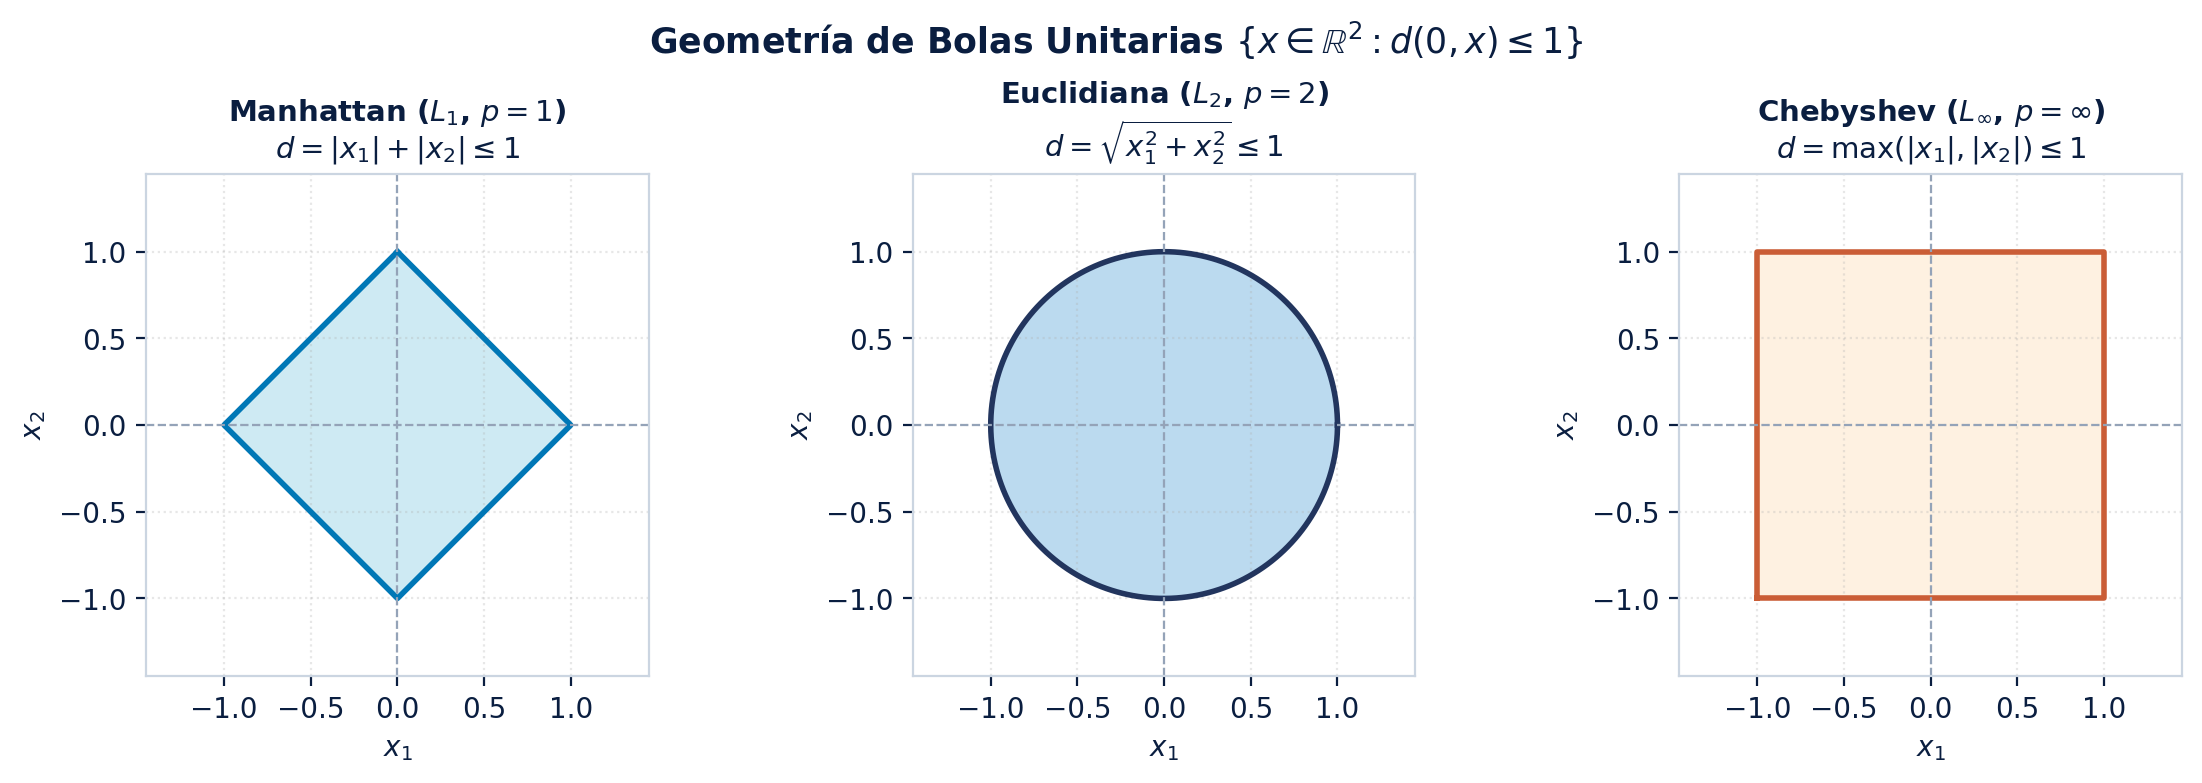
\includegraphics[width=\linewidth]{fig_distancias_knn.png}
\end{column}

\begin{column}{0.36\textwidth}
\begin{contrastbox}{ccdemid}{Lectura Geométrica}
\footnotesize
Bolas unitarias $\{x : d(0, x) \le 1\}$:
\begin{itemize}\setlength{\itemsep}{0.18em}
  \item \textbf{Manhattan ($L_1$):} rombo orientado a $45^\circ$.
  \item \textbf{Euclidiana ($L_2$):} circunferencia perfecta.
  \item \textbf{Chebyshev ($L_\infty$):} cuadrado ortogonal.
\end{itemize}
\end{contrastbox}

\vspace{0.10cm}
\begin{ccdebox}
\scriptsize
\textbf{Efecto en la frontera}: al pasar de $L_2$ a $L_1$ o $L_\infty$, las fronteras de decisión se vuelven poligonales.
\end{ccdebox}
\end{column}
\end{columns}
\source{Figura reproducible generada con Python scikit-learn y matplotlib (CCDE).}
\end{frame}
